\subsection{Without labels (E6)}

The second angle of the project asked whether illicit transactions stand out
\emph{without} labels. The textbook approach, flagging the transactions an
Isolation Forest finds most anomalous, fails completely: PR-AUC
\IFAFUnsupAnomalousPRAUC{} and ROC-AUC \IFAFUnsupAnomalousROCAUC{}, worse than a
random ranking (PR-AUC \UnsBaseRate{}). The anomalies in this network are licit:
all of the 500 most anomalous labelled test transactions are licit, and they are
better connected than average (median degree 5 against 2). Illicit transactions
are \emph{typical} (Fig.~\ref{fig:anomaly}): they look like the bulk of ordinary
payments, consistent with their simple shape (at most three outputs,
Section~3). Fitting the forest on known licit transactions only does not change
this.

Inverting the rule, flagging the \emph{most typical} transactions, turns the same
forest into a useful detector: PR-AUC \IFAFUnsupTypicalPRAUC{} and ROC-AUC
\IFAFUnsupTypicalROCAUC{}, still with no label used for fitting. The direction is
one bit of domain knowledge, and it is the opposite of the usual assumption.

\begin{figure}[t]
  \centering
  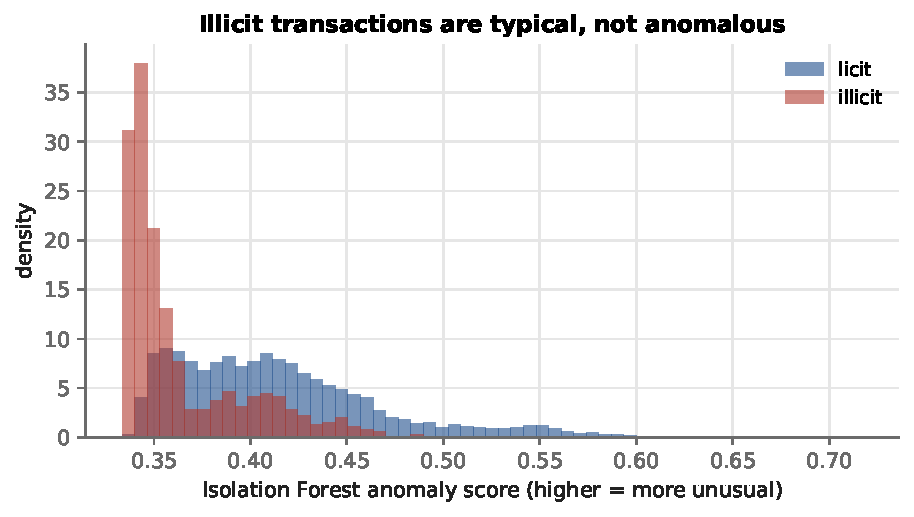
\includegraphics[width=\columnwidth]{../reports/figures/e06_anomaly_scores.pdf}
  \caption{Isolation Forest anomaly scores of labelled test transactions.
  Illicit transactions sit at the \emph{least} anomalous end.}
  \label{fig:anomaly}
\end{figure}

How many labels are worth more than that bit of knowledge?
Fig.~\ref{fig:labeleff} trains XGBoost on random subsets of the labelled training
data. With \LabelEffNA{} or \LabelEffNB{} labels it is below the label-free
detector; from about \LabelsToBeatIF{} labels on it is above it. With
\LabelEffNE{} labels it reaches \LabelEffE{}, and the remaining 29,000 labels add
less than 0.1 PR-AUC (\LabelsFullPRAUC{} with all of them). Labels are very
valuable at first and then quickly saturate. Better labels \emph{of the right
period} would help more than more labels (Section~\ref{sec:drift}).

\begin{figure}[t]
  \centering
  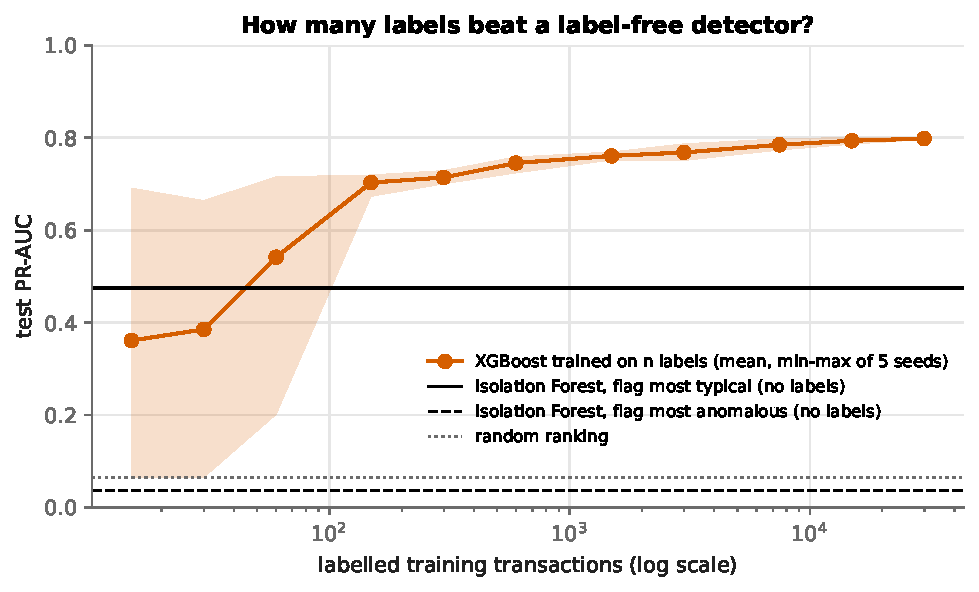
\includegraphics[width=\columnwidth]{../reports/figures/e06_label_efficiency.pdf}
  \caption{Test PR-AUC of XGBoost trained on $n$ random labelled transactions,
  against two label-free Isolation Forest rules.}
  \label{fig:labeleff}
\end{figure}

\subsection{What the model relies on (E8)}

SHAP values~\cite{lundberg2017} of XGBoost trained on AF+G attribute
\ShapLocal{} of the total importance to the 93 local features, \ShapAgg{} to the
72 aggregated ones and \ShapStruct{} to the nine structural features
(Fig.~\ref{fig:importance}). Shuffling each group on the test set confirms the
order and sharpens it: PR-AUC drops by \PermLocal{} without the local features,
\PermAggregated{} without the aggregated ones and \PermStructure{} without the
structure. The aggregated features get a large SHAP share but are partly
redundant with the local ones (correlation, Section~3); the model can fall back
on local information when they are shuffled, but not the other way round. The
group shares are the same before and after the shutdown, so the model does not
switch to different evidence when it starts to fail.

\begin{figure*}[t]
  \centering
  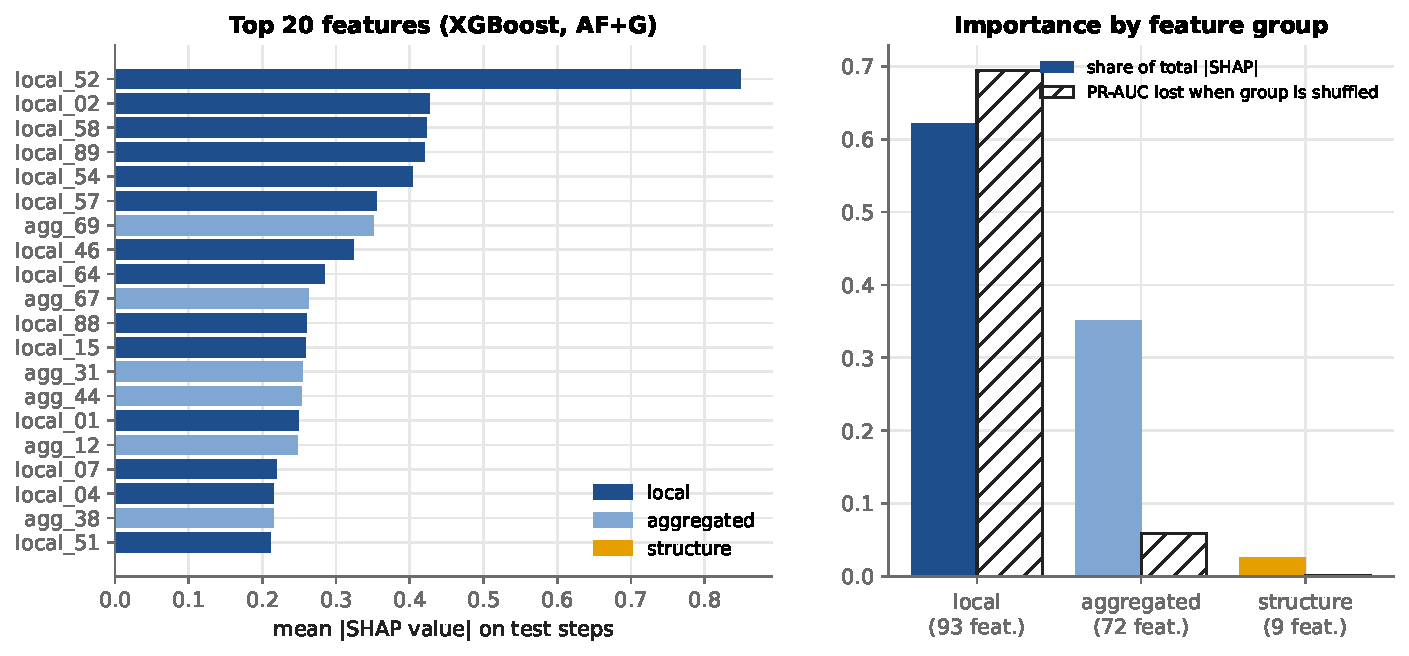
\includegraphics[width=0.85\textwidth]{../reports/figures/e08_importance.pdf}
  \caption{Left: the 20 features with the largest mean $|$SHAP$|$ (XGBoost,
  AF+G). Right: importance per feature group, as a share of total $|$SHAP$|$ and
  as the PR-AUC lost when the whole group is shuffled.}
  \label{fig:importance}
\end{figure*}
